\documentclass[12pt, A4paper, english]{book}
\usepackage{amsfonts}
\usepackage{amsmath}
\usepackage{amssymb}
\usepackage{amsthm}
\usepackage{babel}
\usepackage{color}
\usepackage{float}
\usepackage[T1]{fontenc}
\usepackage{graphicx}
\usepackage[colorlinks]{hyperref}
\usepackage[utf8]{inputenc}
\usepackage{listings}
\usepackage{textcomp}
\usepackage[style=ieee]{biblatex}
\usepackage{tabularx}

\makeatletter
\def\@makechapterhead#1{%
	\vspace*{50\p@}%
	{\parindent \z@ \raggedright \normalfont
		\ifnum \c@secnumdepth >\m@ne
		\if@mainmatter
		%\huge\bfseries \@chapapp\space \thechapter
		\Huge\bfseries \thechapter.\space%
		%\par\nobreak
		%\vskip 20\p@
		\fi
		\fi
		\interlinepenalty\@M
		\Huge \bfseries #1\par\nobreak
		\vskip 40\p@
}}
\makeatother

\addbibresource{bibliography.bib}

\definecolor{dkgreen}{rgb}{0, 0.6, 0}
\definecolor{gray}{rgb}{0.5, 0.5, 0.5}
\definecolor{daynineyellow}{rgb}{1.0, 0.655, 0.102}
\definecolor{url}{rgb}{0.1, 0.1, 0.4}

\lstset{frame=tb,
	language=python,
	aboveskip=3mm,
	belowskip=3mm,
	showstringspaces=false,
	columns=flexible,
	basicstyle={\small\ttfamily},
	numbers=none,
	numberstyle=\tiny\color{gray},
	keywordstyle=\color{blue},
	commentstyle=\color{daynineyellow},
	stringstyle=\color{dkgreen},
	breaklines=true,
	breakatwhitespace=true,
	tabsize=3
}

\lstset{inputpath="C:/Users/Torstein/Documents/skole/USN/IIA2017/Assignment 4/"}
\graphicspath{{C:/Users/Torstein/Documents/USN/IIA2017/Assignment 4/}}
\hypersetup{colorlinks, linkcolor = black, urlcolor=url}

\author{08/03-24, Torstein Solheim Ølberg 263054}
\title{Multitasking and Real-time DAQ simulator}
\date{}

\addto\captionsenglish{\renewcommand{\contentsname}{Table of Contents}}

%\lstinputlisting{Filnavn! type kodefil}. Use [linerange=0-73] or [linerange=73-] to crop
%\includegraphics[width=12.6cm, height=8cm]{Filnavn! type png}

\begin{document}
\maketitle
\tableofcontents

	\chapter{Introduction}
\label{sec:Intro}
Many Data Acquisition (DAQ) simulators have been created \cite{a1}\cite{a2}\cite{a3}, with a different goals extents. Thus far however, all DAQ simulators have relied on a single task performing all the work and not taken use of computers multiple cpu cores. In this report a DAQ simulator with the capabilities of multitasking the collection of values will be presented. \\
First the report will present some relevant theory on multitasking and real-time systems, useful for understanding the final application. Then an example of a multitasking system with properties as shown in figure \ref{im:params} \cite{app}, will be presented and evaluated to give more perspective on the challenges of such a system. Then a fictional real-time system will be presented and a control system from the selection presented in figure \ref{im:ROTSparams} will be chosen. Finally, the DAQ simulation device will be presented, evaluated and a conclusion of the results and work on the project will be drawn. A flowchart of the DAQ device can be found in Appendix A. The complete code of DAQ simulator can be found in Appendix B.
		\begin{figure}[H]
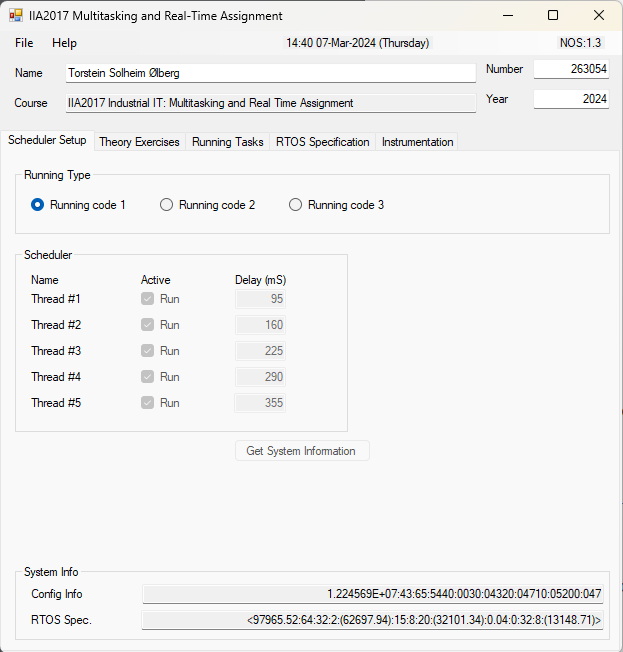
\includegraphics[width=\linewidth, height=15cm]{Parameters_1.png}
\caption{The parameters of the multitasking system to be studied. There are 5 threads running, and three different possible codes.}
\label{im:params}
		\end{figure}
	
	\chapter{Method}
		\section{Theory}
\label{subsec:Theory}
A small background on real-time and multitasking systems is useful to better understand these systems, and the set of questions seen in figure \ref{im:theory} has been chosen alongside the discussion of an example of one of each such systems to bridge this gap for any readers. 
			\begin{figure}[H]
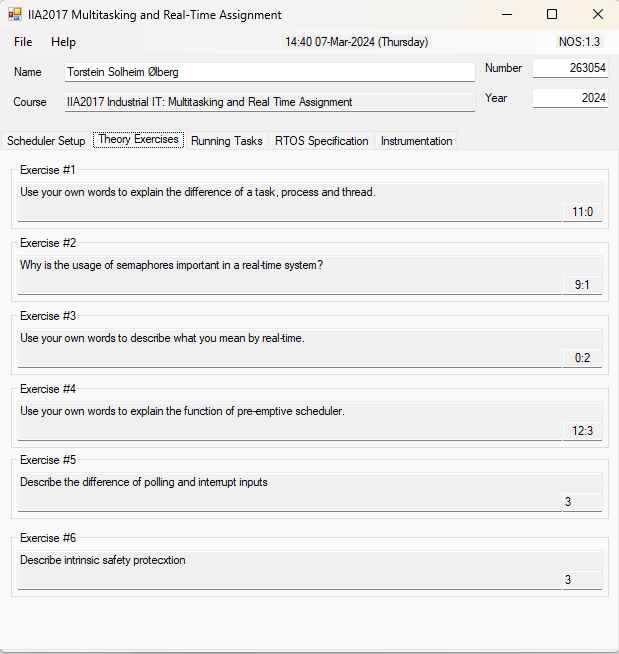
\includegraphics[width=\linewidth, height=15cm]{Parameters_2.png}
\caption{The questions chosen to give a short background for multitasking and real time systems. There are 6 questions in all, asking for explanations to different concepts.}
\label{im:theory}
			\end{figure}

			\subsection{Question 1}
A process is a program running on a large microprocessor which uses a memory management unit and a logical memory area to control its memory access. It is great at keeping its jobs separate from other processes, because only it has access to its memory, but must use extra operating system services to exchange data with other processes if this is needed \cite{LN}. \\
A thread is a subprocess, started by a process to perform some small but time consuming task. It shares the data memory area with all other threads, and the process, but has its own code memory which allows it to work separately \cite{LN}. \\
A task is a program running on smaller microprocessors which does not use memory management units, and uses the physical memory directly. This means, in contrast to the process, that it has access to all other tasks memory and can easily exchange data, but also that it can easily disrupt other tasks and that memory access synchronisation is important when working with them \cite{LN}.
		
			\subsection{Question 2}
Since a semaphore is a variable used to signal between different actors to solve synchronisation problems, and real-time systems needs to solve synchronisation in some way, semaphores are important to these systems \cite{LN}.
		
			\subsection{Question 3}
Real-time means that something is interacting with the world and thus has to take into account the worlds timeline. In relation to software and hardware, this means a system that monitors some real world system and must be able to use this systems status within some time interval \cite{LN}.
		
			\subsection{Question 4}
A pre-emptive scheduler is tasked with deciding what task should be run at the moment, based on the priority of the task. It does this by regularly checking which is the task with the highest priority, stopping any already running tasks and saving their state, and starting the most important task. This is in contrast with the non-preemptive one, which allows the running task to finish and then assigns the next task \cite{LN}.
		
			\subsection{Question 5}
When a system should be capable of handling events, it has to know which event has happened and when it happens. Polling and interrupt inputs are two solutions to this problem. Polling means the system itself checks if an event has occurred regularly, using resources to check the state of an event. Interrupt input however bases the detection on the event sending a signal itself, telling the system an event has occurred and that it needs to stop and deal with this \cite{LN}.
		
			\subsection{Question 6}
Intrinsic safety protection is a signalling technique for electrical equipment to be used in hazardous areas. If equipment properly follow this criteria, the can be approved for use in all zones, and this is the only option for using electrical signals in zone 0. The basis for the technique is to limit the energy for electrical signals and surface temperature such that they are unable to ignite anything. This is done by limiting the voltage of any equipment in a hazardous area, and if necessary include fail safes which will cut the power at to high voltage. Since the equipment is safe by design, there is usually no need for any other safety regulations \cite{LN}.

		\subsection{Real-time System}
The real-time system presented by Skeie \cite{task} with the properties as seen in figure \ref{im:params} can be run using the application also produced by Skeie \cite{app} It consists of an application with three codes, each of which starts 5 threads. Each thread performs 6 steps, before starting again at step 1. 5 of the six steps use shared resources with the other threads, where these resources are different data stored, the current time, and the display of the application. This evaluation will disregard the computer memory resource, and cpu use, and focus on the display. Each thread is started and attempts to collect the current time from the computer. The first one to collect will release the current time giver and request the display so it can print its ID and the time to the display. This process will continue for all threads and the five first steps, printing the name, year, number and a new line character. Then the thread performs a delay given in figure \ref{im:params}, and starts over again. \\
An application, like this, which performs multiple tasks and scheduling each to use a shared resource one at a time will be affected by this sharing of resources. A Windows system scheduler normally performs a check every 20 ms \cite{LN} to check if it is performing the most important task, and then reassigns resources accordingly. It also does this when a resource is available, allowing for changes faster than every 20 ms. This application will as a result have bottlenecks for the threads at the use of the printer, since this is a resource used by all the threads at almost all the steps. Only the delay step can be performed simultaneously and will ensure the threads occupation of the printer will eventually spread out. \\
The first code of \cite{app} produces a result included in figure \ref{im:runtimestart1} and \ref{im:runtimestop1}. These figures show only the start and stop of the results, however they give an indication of the rest of the printout. 
				\begin{figure}
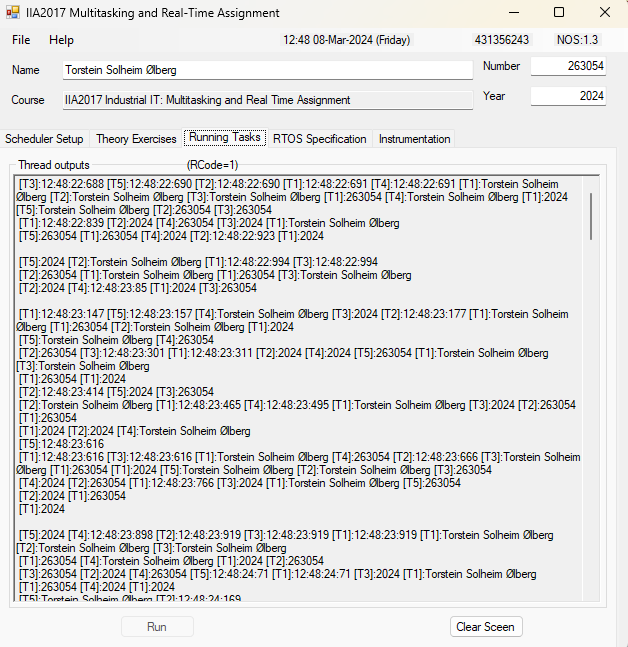
\includegraphics[width=\linewidth]{Runtime_start1}
\caption{The start of code one's printout. Each thread prints with the start of the message being the threads id.}
\label{im:runtimestart1}
				\end{figure}
				\begin{figure}
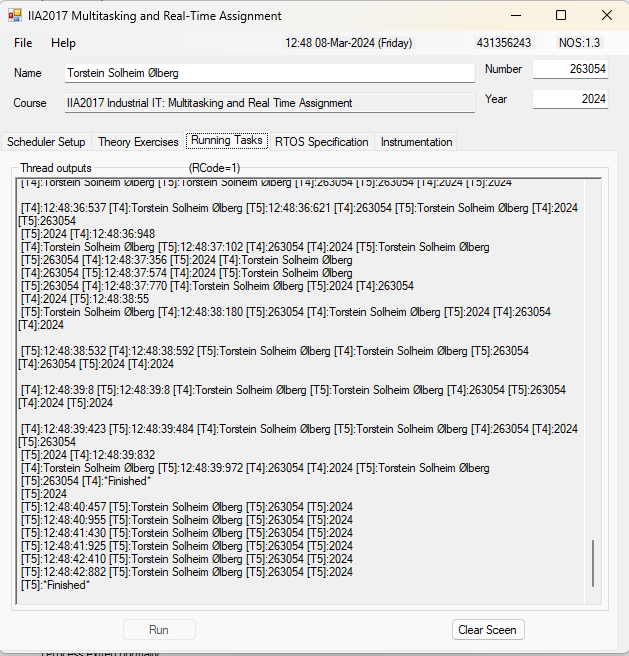
\includegraphics[width=\linewidth]{Runtime_stop1}
\caption{The end of the first codes printout. At the end of the printout, the fifth thread is finished.}
\label{im:runtimestop1}
				\end{figure}
Each thread performs the loop 43 times, and the runtime for the first thread is about 6 seconds and 500 ms. All other threads had a runtime longer than this one, and the main factor for how long time the threads used where the delays. However, with a delay of 95 ms and looping for 43 times and assuming the time to actually perform the steps is negligible, the time it would take for only thread one to run would have been four seconds and 85 ms. The extra time used in waiting for the resources to be available thus accounts for about a third of the time used. The fifth thread used 20 seconds and 192 ms, and using the same assumptions as for thread one, it should have used 15 seconds and 265 ms. This is a much longer time, but comparatively, it uses a lot less of its time waiting for resources. This is a result of the other threads finishing before it and as a result the thread has fewer other threads to wait for. The other three threads have runtime in between these two, with a decreasing amount of the time as a result of the waiting. \\
Running code 2, a very different result is produced. In figure \ref{im:runtimestart2} and \ref{im:runtimestop2} the displayed results show that each of the threads run a full loop before giving up the printer resource to another thread. 
				\begin{figure}
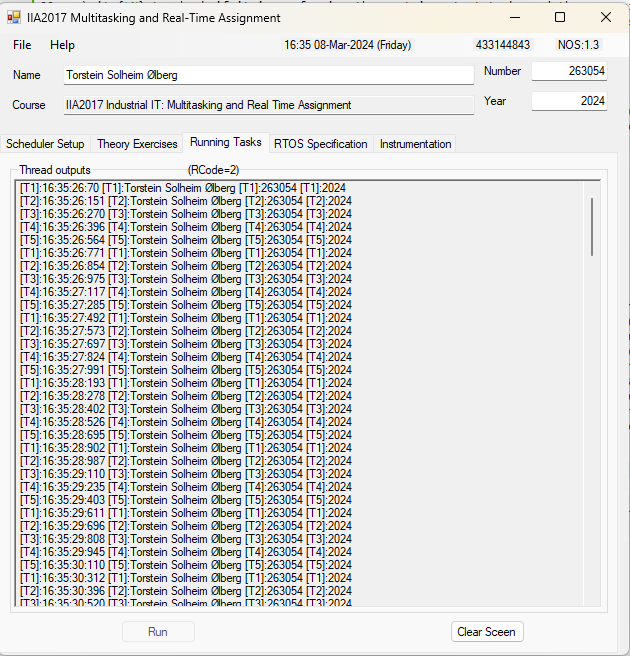
\includegraphics[width=\linewidth]{Runtime_start2}
\caption{The start of code twos printout. This code produces a much more organized result than code 1 did.}
\label{im:runtimestart2}
				\end{figure}
				\begin{figure}
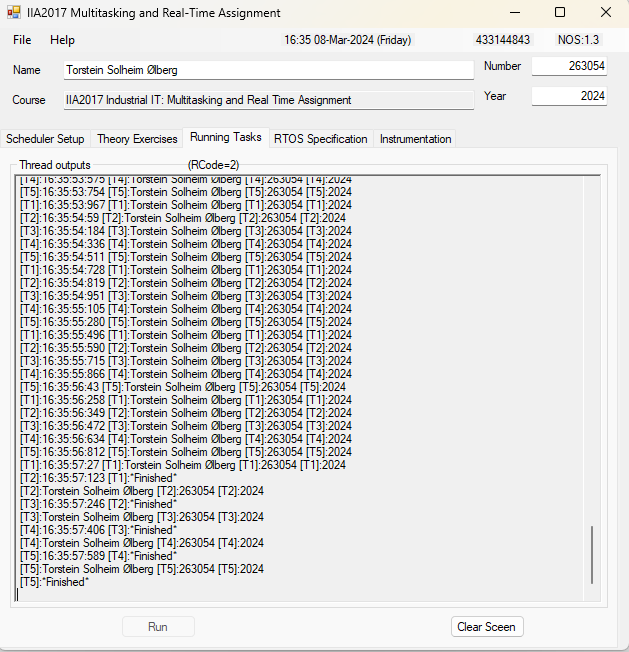
\includegraphics[width=\linewidth]{Runtime_stop2}
\caption{The end of code twos printout. All threads finish in order ant at almost the same time.}
\label{im:runtimestop2}
				\end{figure}
However, the number of loops are the same, and the runtime for thread one is 30 seconds and 570 ms. This is a lot longer than the first code, and the reason is that all the threads wait for each other and all loops are performed in sequence. This means that all threads have to wait for the other threads to have finished their uses of the resources and also that thread one has to wait for the delay of thread five to finish and it to have performed its steps before it can get the display resource again. The runtime of thread five is 31 seconds and 25 ms, which is also longer than in code 1, but is almost the same as thread 1. The other threads have runtime in between the first and fifth as earlier. \\
Running the final, third, code the printout starts in the same way as the last one. However, after five loops from all the threads, the printout changes, as seen in figure \ref{im:runtimestart3} and \ref{im:runtimestop3}, to only each of the threads until they have finished in turn of order. 
				\begin{figure}
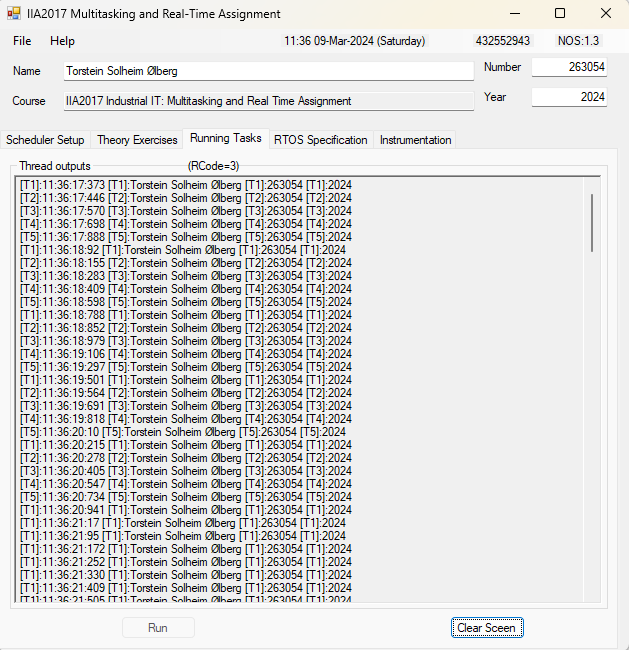
\includegraphics[width=\linewidth]{Runtime_start3}
\caption{The start of code threes printout. There is a change in the pattern just visible at the bottom of the page.}
\label{im:runtimestart3}
				\end{figure}
				\begin{figure}
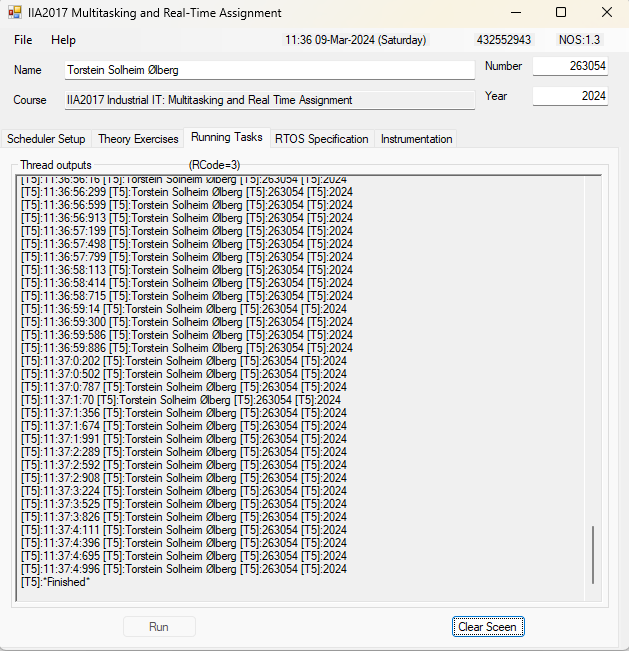
\includegraphics[width=\linewidth]{Runtime_stop3}
\caption{The end of code threes result. Only the fifth thread is still printing anything as the other threads have finished.}
\label{im:runtimestop3}
				\end{figure}
The runtime of thread one is now back to being 6 sec 520 ms almost the same as in the first code. The fifth thread however has a runtime of 47 seconds and 108 ms. These new changes in runtime are a result of this code not mixing the threads actions at all after the fifth loop, and this means all threads have to wait for the threads before them to perform their delays. The other threads have a runtime between the first and the fifth like for the two other codes. \\
This application uses a mutex \cite{task} to organize its common resources. This means it uses a binary variable passed between the thread that is using a resource and which needs to be acquired before a resource can be used. As an alternative, a semaphore could have been used. Here an unsigned integer is used to signal all threads how many of a resource are available. When a resource is acquired, the thread decrease the number of the integer to signal it is using one of the resources, and when a thread releases a resource it increases the integer to indicate a resource is available. For this system however, there is only one printer and this means we would use a binary semaphore. This semaphore is almost the same as a mutex and the printout of the third code would be the same. \\
The three codes prioritise the use of its resources very differently, and this leads to very different runtime and printouts. While the information printed is the same for all three codes, the first code prints everything very unorganized, but also wastes the least time waiting for resources to be available. The second code is more organised, but also wastes more time waiting. Finally, the third code is a bit odd. It starts off the same way as code two, but then switches to an even more organised printout, but this also leads to even more time wasted and a longer run time. The odd behaviour can only be a result of some priority relation lining up with the time of the delays.

		\section{Time requirements}
The control system specified by Skeie \cite{task} needs a Real Time Operating System (RTOS) to work. Given the options for the RTOS specified in the application in figure \ref{im:ROTSparams} \cite{app}, a choice must be made of which is to be chosen.
			\begin{figure}
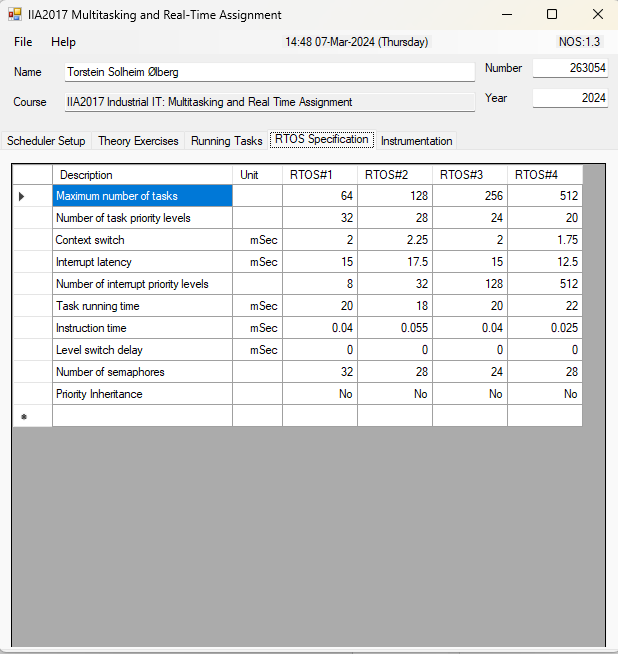
\includegraphics[width=\linewidth]{Parameters_3}
\caption{The four different RTOS available for selection to be used with the control system. They each have different numbers of tasks, levels and time consumptions when performing work.}
\label{im:ROTSparams}
			\end{figure}
			\begin{figure}
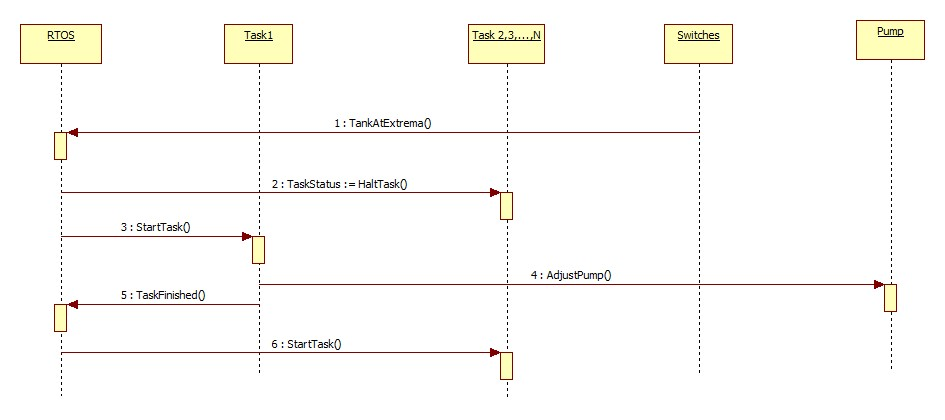
\includegraphics[width=\linewidth]{Timing Diagram.jpg}
\caption{The sequence diagram of a single event of the control system. The interrupt goes of and any other tasks are stopped before the pump is set to a new value and the old task can start again.}
\label{im:TimingDiag}
			\end{figure}
Since a ROTS must contain at least 16 priority levels \cite{LN}, ROTS\#1 is excluded and the others can be chosen. From the calculation of the response time from a switch is activated to the pump state is changed, ROTS\#2 is unattractive as it has a response time of 249.85ms and the required time is 250ms. This limits the options to the two last, and with the highest number of tasks, interrupt levels and lowest response time, ROTS\#4 is chosen to be used.

		\section{DAQ Simulator}
The DAQ simulator is developed in the programming language python. This allows it to use the inbuilt threading capabilities of the threading package \cite{threading}. The parameters used for the application can be seen in figure \ref{im:DAQparams} and an explanation of the requirements are given in the specification \cite{task}.
			\begin{figure}
\centering
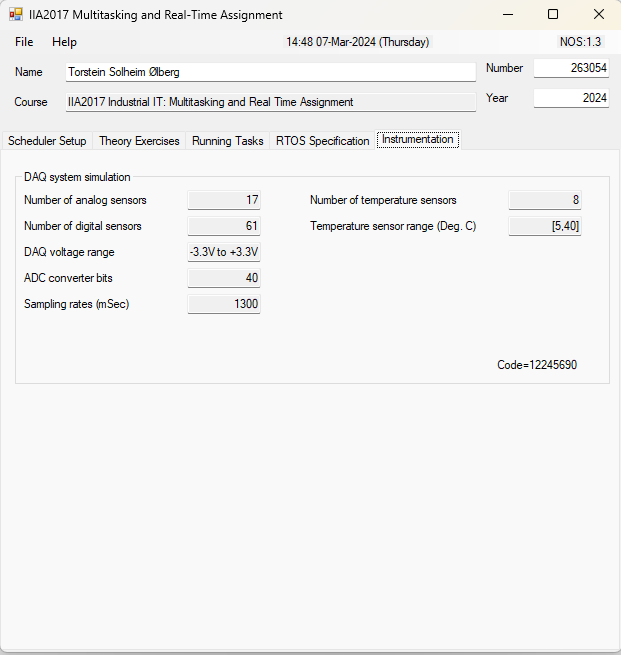
\includegraphics[width=\linewidth]{Parameters_4}
\caption{The configuration parameters for the DAQ simulator application. The number of sensors for the three types are specified, as well as parameters used for determining the resolution of the digital values and the sampling rate.}
\label{im:DAQparams}
			\end{figure}

	\chapter{Results}
The produced application is a python program simulating a DAQ system running at real-time. It sets up at set of threads, each associated with its own sensor and continuously gathers sensor values at specific time intervals until the user prompts it to stop using the return key. The simulated sensors set up their own random number generators, which they use to produce sensor values, and a ADC is simulated to give the sensor values as digital representations of the data to the DAQ system. All data collected is written to the terminal as seen in figure \ref{im:daqterminal} in Appendix A, and also stored in the data.csv file as seen in figure \ref{im:csv}, also in Appendix A. A flowchart of the steps in the application can also be found in Appendix A.
		\begin{figure}
\centering
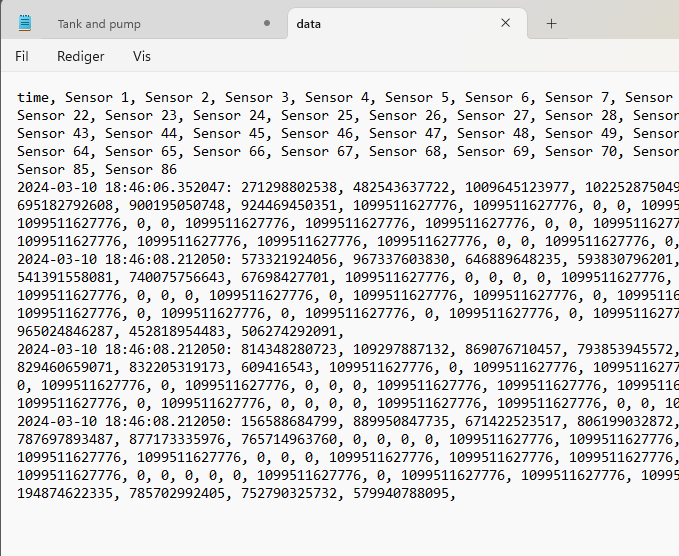
\includegraphics[width=\linewidth]{csv}
\caption{An extract of the results from the DAQ simulator saved to data.csv. Only some of the sensors are visible.}
\label{im:csv}
		\end{figure}
		\begin{figure}
\centering
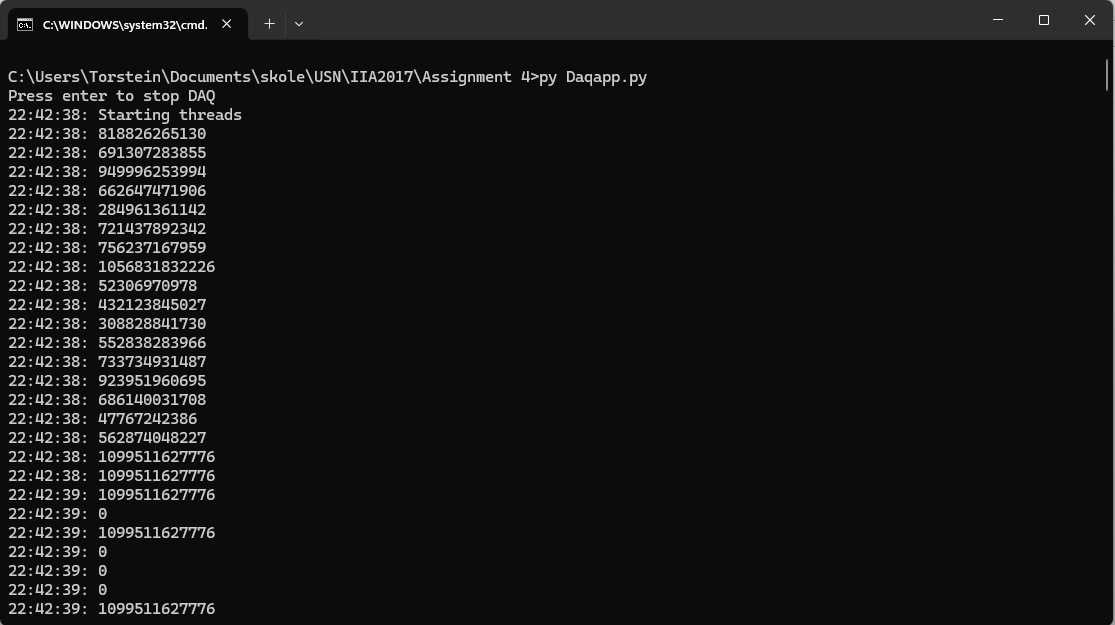
\includegraphics[width=\linewidth]{DAQterminal}
\caption{A screenshot of the interface of the DAQ application. The user is told to press eter to stop the application and after this the results collected by the sensors are written to the terminal along with the time they where collected.}
\label{im:daqterminal}
		\end{figure}
	\chapter{Discussion}
The DAQ simulator is a simple application, fulfilling the goals of the project and the specifications given. It collects and stores multiple sensor values quickly and prints them to the screen faster than the earlier DAQ devices did. This is a result of it performing multiple collections of sensor values at the same time, which is much faster than what a single task system could do. The saving of the data is also done at the same time as the sensors wait for the next interval, which allows for more accurate time intervals and shorter delays. However, the system is fragile because it doesn't implement its own scheduler for each of the tasks, simply trusting the local scheduler of the OS it is run on to control the tasks. This is fine for long time intervals as used in this report, but could be problematic with the addition of to many sensors or the reduction of the sampling time. \\
The application is also a bit to unintuitive, with most of the parameters being coded into the system and problematic for the user to adjust. In the future, it would be useful to implement a possibility for the user to configure the number of sensors of each type, the bit resolution and voltage range, the filename of the csv file and perhaps also the header to use in the file if. This should be possible to do even for someone not learned in the programming language, and the simplest way to do this would be either through command-line arguments, prompted user input, or perhaps the most useful choice would be a GUI.

	\chapter{Conclusion}
The new DAQ simulator, utilising a new an much quicker way of collecting sensor data, has been developed and it fulfils the goal of using multitasking system to collect and save data for multiple sensors at the same time. It is simple, but with further development, like implementing a GUI it could be very useful. \\
The project work was expected to be split evenly among the different parts, as seen in table \ref{tab:eval} under the requirements columns. However, as seen under the Your evaluation column, a lot more work was put into understanding the multitasking system than any of the other parts. The most likely cause of this was the lack of information on the build-up of the system and the very long time in finding the start and end of the first thread in code 1.
		\begin{figure}
\centering
\noindent \begin{tabularx}{\linewidth}{@{}|X|X|X|X|}
\hline
Section 		& Requirements (\%)	& Your evaluation (\%) 	& Comments \\
\hline
Introduction 	& 2					& 2						&  \\
\hline
Theory 			& 26				& 26 					&  \\
\hline
MT System		& 25				& 40 					&  \\
\hline
Time Req.		& 20				& 20					&  \\
\hline
DAQ sim. 		& 25				& 10					&  \\
\hline
Conclusion 		& 2					& 2						&  \\
\hline
Sum				& 100				& 100 					&  \\
\hline
			\end{tabularx}
\caption{A summary of the time used to work with the project, both the expected and the actually used.}
\label{tab:eval}
		\end{figure}

\printbibliography
	
	\chapter{Appendix A}
		\begin{figure}
\centering
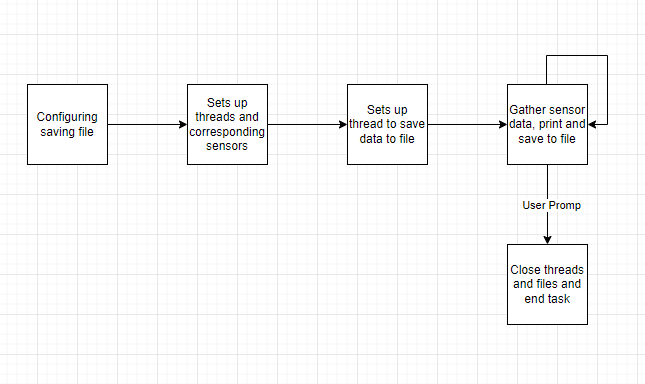
\includegraphics[width=\linewidth]{Flowchart}
\caption{A flowchart of the steps taken by the DAQ application.}
\label{im:flowchart}
		\end{figure}


	\chapter{Appendix B}
Here you can find the code file for Daqapp.py. The whole project can also be found at the github of the project \cite{github}.
\lstinputlisting{Daqapp.py}

\end{document}